\begin{figure*}[htp!]
    \centering
    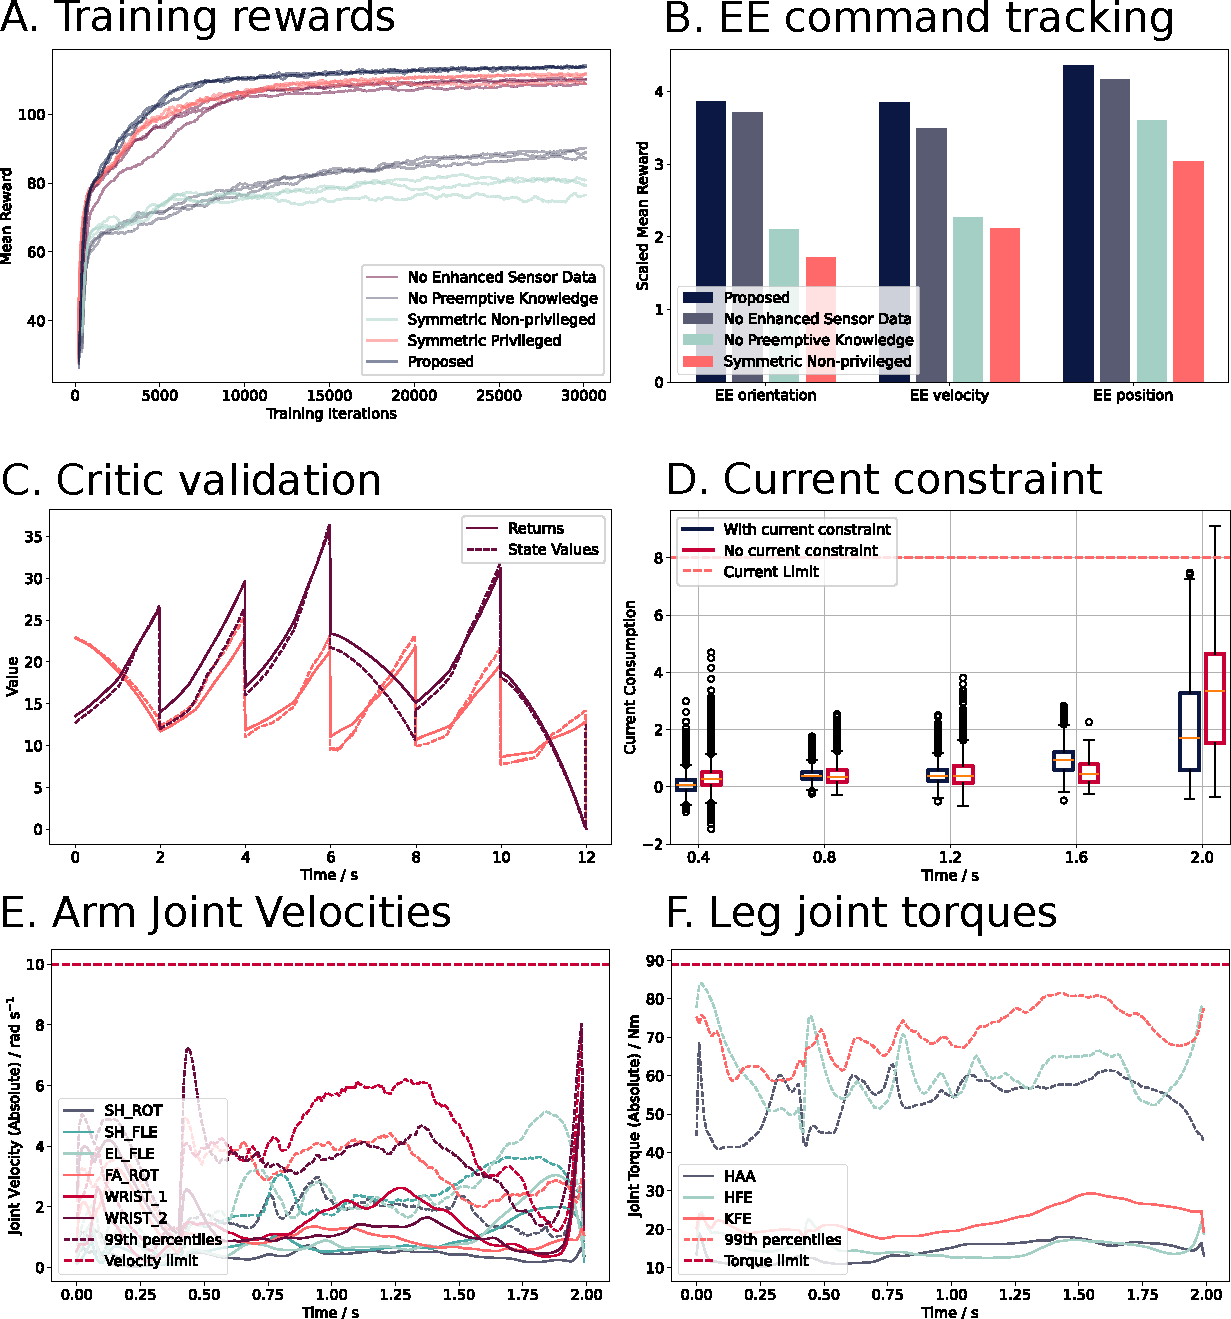
\includegraphics[width=0.9\textwidth]{Figures/MethodValidation/revision_method_validation.pdf}
    \caption{\textbf{Validation of the training method. (A-B)} Ablation studies comparing different observation configurations show that our method consistently outperforms baseline training setups in terms of both convergence time and final end-effector tracking performance. \textbf{(C)} Multiple sample trajectories (represented by different colors) demonstrate that our value prediction closely aligns with the computed trajectory return. \textbf{(D)} The current consumption constraint is respected by policies trained using the N-P3O formulation. \textbf{(E)} The arm joint velocities over the sample swings. \textbf{(F)} The leg joint torques over the sample swings. \textbf{(D-F)} The box and line plots use data from all target positions on the court, each totalling 199,650 trajectories.}
    \label{fig:method_validation}
    
    % \vspace{-1.5em}
\end{figure*}

% add badminton shuttlecock trajectory